\section{Experiments}
\subsection{Synthetic Data Set}
\begin{frame}{Structural Hamming Distances}
$5$ synthetic networks of size $5,7,10,20,50$. (ground truth structures are known.)
\begin{figure}
\vspace{-2cm}
\centering
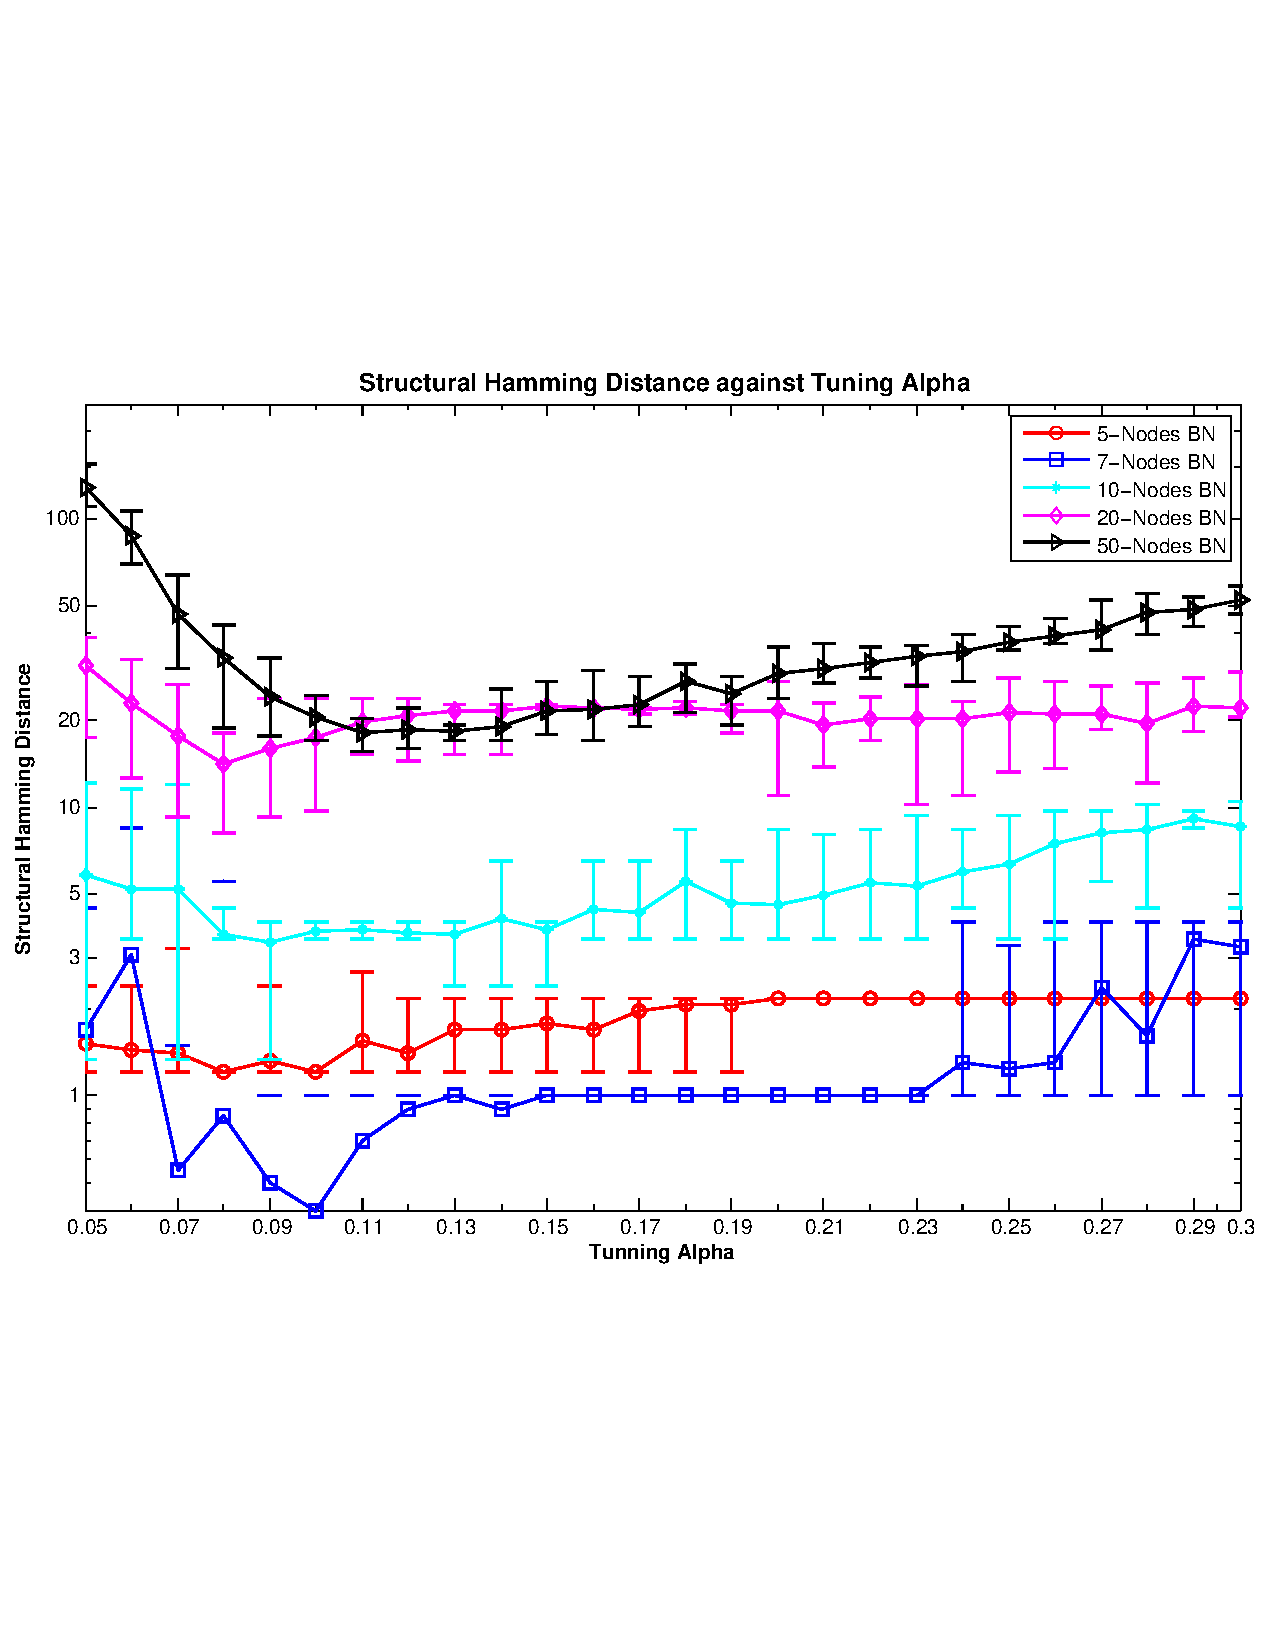
\includegraphics[scale=0.3]{imgs/shd-alpha-errb}
\vspace{-2cm}
\caption{Structural hamming distance (SHD) against threshold $\sigma$}
\end{figure} 
\end{frame}
\begin{frame}{Error rates}
\begin{figure}
\vspace{-2cm}
\centering
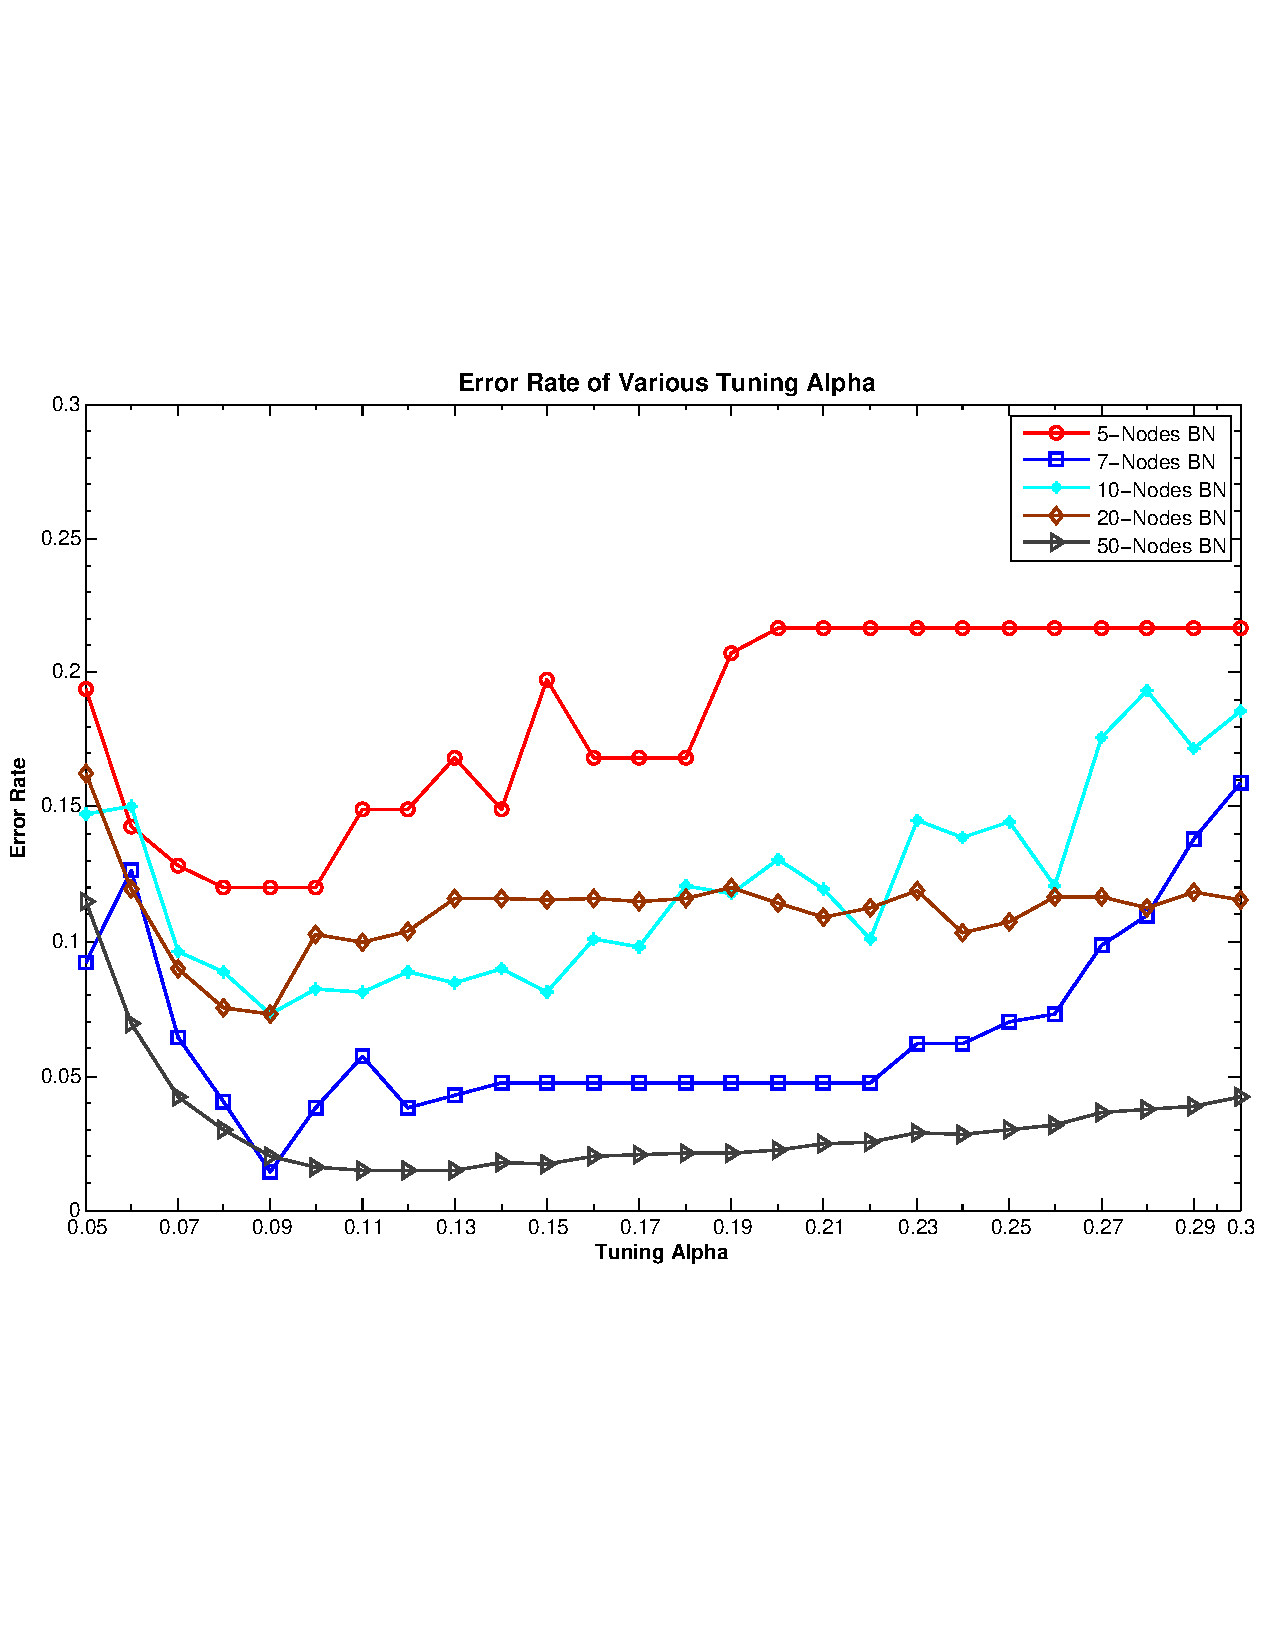
\includegraphics[scale=0.35]{imgs/ErrorRate-copula}
\vspace{-2.2cm}
\caption{Error rates in terms of SHD}
\end{figure} 
\end{frame}
\subsection{Real-world Data Set}
\begin{frame}{Boston Housing Price (UCI Repo.)}
\begin{minipage}[t]{0.45\linewidth}
 \vspace{0pt}
\centering
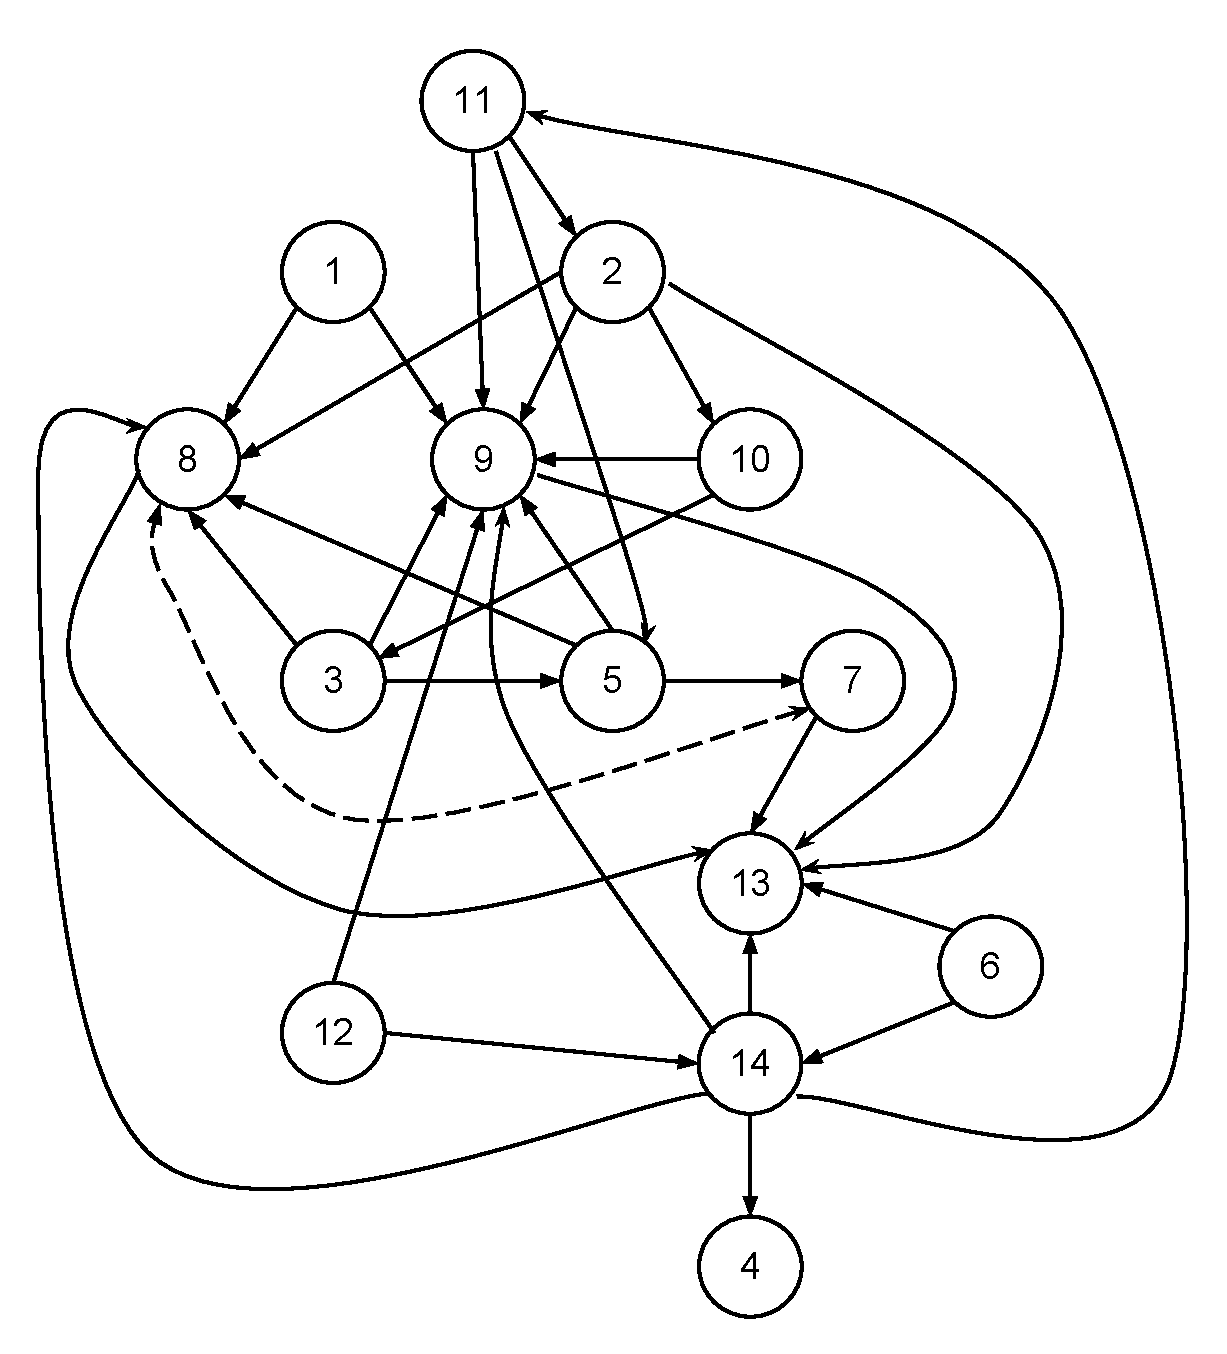
\includegraphics[width=\textwidth]{imgs/BostonHousingNetwork}
\end{minipage}\hfill
\begin{minipage}[t]{0.4\linewidth}
 \vspace{0pt}
\centering
\begin{scriptsize}
\begin{tabular}{|l|}
\hline
The factor names\\
\hline
	1. crime rate by town \\
    2. percent of residential land\\
    3. proportion of non-retail business \\
    4. Resided by Charles River?\\
    5. nitric oxides concentration \\
    6. average number of rooms\\
    7. proportion of built prior to 1940 \\
    8. distances to employment centres \\
    9. accessibility to radial highways \\
    10. property-tax rate\\
    11. pupil-teacher ratio\\
    12. the percent of blacks by town\\
    13. lower status of the population \\
    14. Median value of own homes\\
\hline
\end{tabular}
\end{scriptsize}
\end{minipage}
\end{frame}
\begin{frame}{Abalone Data Set (UCI Repo.)}
\begin{minipage}[t]{0.45\linewidth}
 \vspace{0pt}
\centering
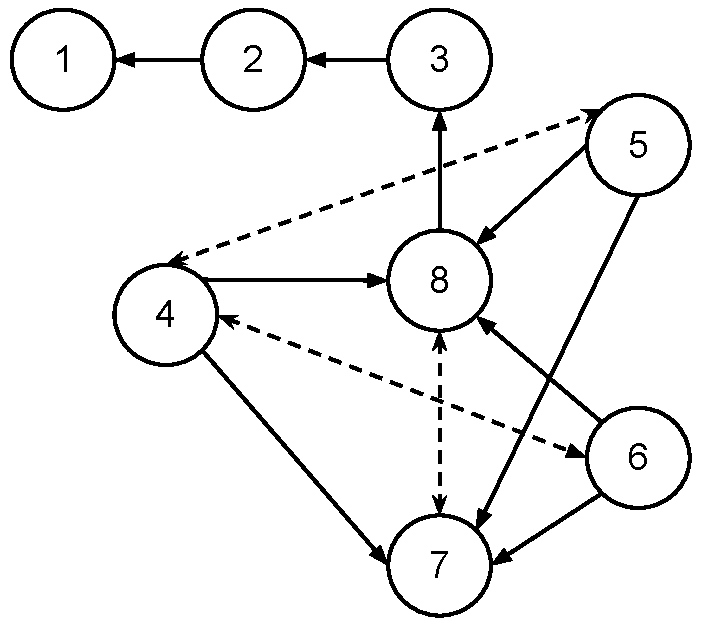
\includegraphics[width=\textwidth]{imgs/AbaloneNetwork}
\end{minipage}\hfill
\begin{minipage}[t]{0.45\linewidth}
 \vspace{0pt}
\centering
\begin{scriptsize}
\begin{tabular}{|l|}
\hline
The factor names\\
\hline
1. Length (longest shell) \\
2. Diameter\\
3. Height (with meat)\\
4. Whole weight  \\
5. Shucked weight (without shell)\\
6. Viscera weight (after bleeding) \\
7. Shell weight \\
8. Rings (indicating age)\\
\hline
\end{tabular}
\end{scriptsize}
\end{minipage}
\end{frame}